\author{Schmied Margaux\\
Galbiati Federica\\
Fissore Davide\\
Venturelli Antoine
}
\newcommand{\exam}{Calculability}
\newcommand{\supervisorone}{Enrico Formenti}
\def\dotminus{\mathbin{\ooalign{\hss\raise1ex\hbox{.}\hss\cr
  \mathsurround=0pt$-$}}}

\title{GUI for RAM programs with \\ parser and interpreter}
\date{2021/2022}

\documentclass[a4paper,12pt]{article}
\usepackage[left=30mm,top=30mm,right=30mm,bottom=30mm]{geometry}
\usepackage{etoolbox} %required for cover page
\usepackage{booktabs}
\usepackage[usestackEOL]{stackengine}
\usepackage[T1]{fontenc}
\usepackage[utf8]{inputenc}
\usepackage{bm}
\usepackage{graphicx}
\usepackage{subcaption}
\usepackage{amsmath}
\usepackage{amsfonts}
\usepackage{mathtools}
\usepackage{xcolor}
\usepackage{float}
\usepackage{hyperref}
\usepackage[capitalise]{cleveref}
\usepackage{enumitem,kantlipsum}
\usepackage{amssymb}
\usepackage[square,numbers,sort]{natbib}
\usepackage[ruled,vlined]{algorithm2e}
\usepackage{listings}
\usepackage{minted}
\usemintedstyle{emacs}
\usepackage{pgfplots}
\pgfplotsset{width=10cm,compat=1.9}
\setlength{\parindent}{0pt}
\usepackage[english]{babel}
\usepackage[T1]{fontenc}
\usepackage{listings}
\usepackage{color}
\usepackage{dirtree}
\usepackage{minted}
\usepackage{simplebnf}
\newcommand\tab[1][1cm]{\hspace*{#1}}

\definecolor{dkgreen}{rgb}{0,0.6,0}
\definecolor{gray}{rgb}{0.5,0.5,0.5}
\definecolor{mauve}{rgb}{0.58,0,0.82}

\bibliographystyle{unsrtnat}

\usepackage[toc,page]{appendix}

\linespread{1}

\newtheorem{theorem}{Theorem}[section]
\graphicspath{{figures/}}

\setlength{\parskip}{0.5em}
\usepackage[most]{tcolorbox}


\makeatletter
\def\maketitle{
  \begin{center}\leavevmode
       \normalfont
       \includegraphics[width=0.6\columnwidth]{images/logo_master.png}
       \vskip 0.5cm
       \vskip 1.5cm
       \rule{\linewidth}{0.2 mm} 
       {\large \exam}\\[1 cm]
       {\huge \bfseries \@title \par}
       \vspace{1cm}
	\rule{\linewidth}{0.2 mm} \\[1.5 cm]

	\begin{minipage}[t]{0.45\textwidth}
		\begin{flushleft} \large
			\emph{Authors:}\\
			\@author
		\end{flushleft}
	\end{minipage}
	\begin{minipage}[t]{0.45\textwidth}
	    \begin{flushright} \large
			\ifdefempty{\supervisortwo}{\emph{Supervisor:\\}}{\emph{Professor:\\}}
			\supervisorone
		\end{flushright}
	\end{minipage}
	\vfill
	{\Large \@date\par}
   \end{center}
   \cleardoublepage
  }
  
 
\makeatother

\begin{document}

\pagenumbering{gobble}

\maketitle

\tableofcontents

\newpage

\pagenumbering{arabic}

\section{Introduction}
For the calculability course, we had to realize a project. This project is a RAM language interpreter. The RAM language is a pseudo code discussed in class with 4 instructions. This project is divided in 3 parts: the parser, the interpreter and the graphics.

\section{About RAM program}
\label{sec:RAM_intro}
A \textit{RAM} program is a program made by :
\begin{itemize}
    \item a potentially infinity memory with three main registers
    \begin{itemize}
        \item the \textit{memory counter ($R_C$)} which allows to know at each moment what is the current instruction to be executed. If $R_C$ is $0$ or a integer bigger then the number of instructions of the code, the program execution will stop 
        \item \textit{$R_0$} the first register of the memory representing the input of the program
        \item \textit{$R_1$} the second register which can be seen as the case of the memory containing the output of our program
    \end{itemize}
    \item 4 instructions :
    \begin{itemize}
        \item $R_k = R_k + 1$ which increases the value stock in the register $k$ by one
        \item $R_k = R_k \dotminus{} 1$, same as previous instruction, but the value is decreased by one (NB : if the value in $R_k$ is equal to 0, we have that $0 \dotminus{} 1 = 0$ since RAM machines work in $\mathbb{N}$ number set
        \item $IF \; R_k \neq 0 \; THEN \; GOTOB \; n$ means that if the register $k$ does not equal $0$ then $R_C = R_C \dotminus{} n$ (here, as before the subtraction is done as follow $A \dotminus{} B = max(0, A - B)$
        \item $IF \; R_k \neq 0 \; THEN \; GOTOF \; n$ which makes the following operation : $R_C = R_C + n$
    \end{itemize}
\end{itemize}

With a RAM program, as demonstrated in course, it is possible to code all the programs we usually code with any other programming language such as \textit{Python, C, Java, etc.} 

Another important aspect of RAM program we should consider is that, thanks to its infinite registers and the fact that efficiency time of programs is not taken, this program model can be reused and adapted to every new programming language.

Finally working only in $\mathbb{N}$ does not restrict RAM programs, since in fact $\mathbb{Z}$, $\mathbb{Q}$ and  $\mathbb{R}$ can be seen as an extensions of $\mathbb{N}$.

\newpage
We can also introduce some predefined and useful macros, such as, \textit{rp} and \textit{lp} (resp. for \textit{right\_part} and \textit{left\_part}), allowing to treat the value of a register as a \textit{Cantor's couple} (see \ref{sec:cant_pair_func}), this let you pass a variable number of parameters.\\
For example, if you have a program that calculate the sum of $x$ and $y$ then you will put $n$ that is $cantor(x,y)$ in $R_0$.
\\Other two macros are \textit{push} and \textit{pop} which respectively push and pop the value from a register $k$ to a very big register that normally should not be used by the program (we have chosen the $2^{64}$ register).


\section{Design choices}

\subsection{Choice of tools}

\begin{itemize}
\item Technologies : \textbf{Python3.9.9}\\
To realize this project we used the following libraries:
    \begin{itemize}
        \item ply==3.11 (For the parser)
        \item tkhtmlview==0.1.0 (For the help)
    \end{itemize}
\end{itemize}

\subsection{Installation}

You can use the file \textbf{install.sh}

\begin{verbatim}
$ chmod u+x install.sh
$ ./install.sh
\end{verbatim}
Or

\begin{verbatim}
$ python3 -m pip install -r requirements.txt
\end{verbatim}

\section{Integers as instructions or programs}

\subsection{Integer representation}
When we deal with RAM program, as said in Section~\ref{sec:RAM_intro}, we do not treat subtraction as if we were in $\mathbb{Z}$ or other set of number including $\mathbb{Z}$, we are supposed to be in the natural number world. 

In a RAM program subtraction is represented by the $\dotminus$ symbol giving us an expression of the type $A \dotminus B = max(0, A - B)$ therefore the we created the \textit{Int} class that extends the \textit{int} class and overrides the \textit{\_\_sub\_\_} function as shown in Listing \ref{listing:int_class_sub} .

\begin{lstlisting}[
    caption={The Int class}, 
    label={listing:int_class_sub},
    language=Python,
    backgroundcolor=\color{gray!10},
    frame=lines,
    ]
class Int(int):
    def __sub__(self, x: int):
        return Int(max(int(self) - x, 0))
    ...
\end{lstlisting}


\subsection{Gödelisation function}
As seen in course every instruction can be represented as an integer, thanks to Gödel bijective function (look at listing~\ref{god_enc}).

\begin{lstlisting}[
    caption={Gödel encoding function}, 
    label={god_enc},
    mathescape, 
    frame=lines,
    backgroundcolor=\color{gray!10}, breaklines=true
    ]
    $Rk =  Rk + 1 \rightsquigarrow 3 \times  k$ 
    $Rk =  Rk - 1 \rightsquigarrow 3 \times  k + 1$
    $IF\;Rk \neq  0\;THEN\;GOTOB\;n\;\rightsquigarrow 3 \times  [k, [1, [n, 0]]] + 2$ 
    $IF\;Rk \neq  0\;THEN\;GOTOF\;n \rightsquigarrow 3 \times  [k, [0, [n, 0]]] + 2$
 Where : 
    - k is the register number
    - is the number of jump to do inside a if
\end{lstlisting}

\newpage
\subsection{Gödel inverse function}
When we are given an integer and we know that it is an instruction, we can easily decode it with modulo operations (look at listing~\ref{god_dec}).
\begin{lstlisting}[
    caption={Gödel decoding function}, 
    label={god_dec},
    mathescape, 
    frame=lines,
    backgroundcolor=\color{gray!10},
    ]
if $X \equiv 0 \mod 3 \rightsquigarrow$ we have a $Rk = Rk + 1$ instruction
if $X \equiv 1 \mod 3 \rightsquigarrow$ we have a $Rk = Rk - 1$ instruction
  in both cases, k is equal to $\lfloor X/3 \rfloor$
if $X \equiv 2 \mod 3 \rightsquigarrow$ we have a jump instruction
  where $X' =  \lfloor X/3 \rfloor$ and we can decode $X$ in $[k, [j, [n, 0]]]$ 
  with Cantor inverse function (see next paragraph)
\end{lstlisting}
Decoding an instruction like can be done by the \textit{decode\_int\_instr} in \textit{decode\_int.py} file.

\subsection{Cantor pairing function}
\label{sec:cant_pair_func}
Now, we know how to code an instruction, we can so code a program, that is a list of instruction, thanks to Cantor function (look at listing~\ref{cant_enc})

\begin{lstlisting}[
    caption={Cantor encoding function}, 
    label={cant_enc},
    mathescape, 
    frame=lines,
    backgroundcolor=\color{gray!10},
    ]
    $[x, y] = \frac{(x + y) \times (x+y+1)}{2} + y + 1 = n$
    if b is a couple, we encode it at first,
    and that recursively until the last tuple
\end{lstlisting}

The encoding of two integer to a Cantor's int is made by the \textit{cantor} method of the \textit{Int} class.

\subsection{Cantor inverse function}
The Cantor inverse function is not as simple as computing the Gödel inverse one. The Cantor Pairing function is a \textit{Diophantine equation} (voir definition at ...) and finding back the two variables $x$ and $y$ from $n$ ask to iterate from 0 the n to find an intermediate $n'$.  

Since $n$ may be very big, (it is the case if we encode multiple instructions) this task may become very slow, therefore, to speed it, we make a \textit{binary search} to have an answer in a logarithmic time instead of a linear one. 

The decoding function of a Cantor's int to a couple of the form $(x_1, (x_2, (..., (x_n, 0))))$ is made by the \textit{Int} class with the \textit{int\_to\_couple} method.
\newpage
\begin{lstlisting}[
    caption={Cantor decoding function}, 
    label={cant_dec},
    frame=lines,
    backgroundcolor=\color{gray!10},
    language=Python
    ]
class Int(int):
    ...
    def cantor_inv(self):
        tmp = self.aux()
        r = self - ((tmp - 1) * tmp / 2 + 1)
        l = tmp - r - 1
        return l, r
    
    def int_to_couple(s):
        res = Int(s).cantor_inv()
        return res if res[1] == 0 
               else (res[0], Int(res[1]).int_to_couple())
    ...
\end{lstlisting}

\section{Pre-processing}
\subsection{Include}
You have the possibility to include a file. Like the C language, just
write \textit{\#include filename} where '\textit{filename}' is the path of the file you want embedded.
At the pre-processing phase, each line which contain such this instruction will be replace by the content of the precise filename. If the path doesn't exist, an error
(that will not interrupt the execution) will be raised.

\subsection{Define}
This interpreter also offered the possibility of using the \textit{\#define name thing} instruction. Therefore, all '\textit{name}' will be replaced by '\textit{thing}' in the file

\subsection{Some precisions}
When you go to execute the file, you will not see your file modified by the preprocessing instructions, they will be done internally. However, you always have the option to do it manually to see it in \textbf{Tools} -> \textbf{Apply Preprocessing}. The current file will then be modified.

\section{Parser}
\label{sec:parser}
The first step of our RAM interpreter is to parse the instructions. At first we tried to use \textbf{ANTLR4}, it's a parser generator for reading, processing, executing, or translating structured text. Margaux having already used it, it seemed to be a good choice to make the parsing, but once most of the grammar was done, we had a problem.

When we wanted to add the name of the macros and each instruction was detected as a string caused by a priority action problem. Therefore, we started to seek for a solution and we found a Python library named \textbf{PLY} that was easier to use and seemed to solve our problem.

\textbf{PLY} is a Python implementation of the lex and yacc tools commonly used to write parsers and compilers. The parsing is based on the same \textbf{LALR} algorithm used by many yacc tools. \textbf{LALR} parser is a simplified version of an \textbf{LR} parser, for parsing text according to a set of production rules specified by a formal grammar for a computer language. \textbf{LR} is left-to-right derivation.

Our parser detects 10 main kind of grammar rules.

\begin{lstlisting}[
    caption={Detected instruction}, 
    label={detected_instruction},
    mathescape, 
    frame=lines,
    backgroundcolor=\color{gray!10}, breaklines=true
    ]
    0. Rk = Rk + 1
    1. Rk = Rk - 1
    2. if Rk != 0 then gotob n
    3. if Rk != 0 then gotof n
    4. push Rk
    5. pop Rk
    6. rp(Rk, Rl)
    7. lp(Rk, Rl)
    8. begin macro <name> (Rk, Rl, ..., Rz)<code> end macro;
    9. <name> (Rk, Rl, ..., Rz)
\end{lstlisting}

\subsection{Lexical analysis}
The first step of our parser is to make the lexical analyse which verifies if the used vocabulary is correct. We have decided to allow only lower case letters except for the \textbf{R} in registers which can only be capitalized.

So we detected all the words that would be useful to us in addition to the strings for the names of the macros and the numbers for the registers.

\newpage
\subsection{Syntactic analysis}

The creation of grammar \ref{grammar} took longer than expected. It syntactic analysis verifies that the arrangement of words is coherent. We had to create a redundant grammar because the instructions to be parsed in the macros and outside are very similar. For example, in macros, we can have registers with a not known value (a register with name \textbf{$R_x$} is authorized inside a macro definition but not outside).

\subsection{Semantic analysis}
The semantic analysis verifies that the instructions have a meaning else we raise an error. 

In listing \ref{semantic_rules} the number associated with the instructions is the same as in listing \ref{detected_instruction}.

\begin{lstlisting}[
    caption={Semantic rules}, 
    label={semantic_rules},
    mathescape, 
    frame=lines,
    backgroundcolor=\color{gray!10}, breaklines=true
    ]
    1. The instructions 0 and 1 must add and subtract 1.
    2. The instructions 2 and 3 must compare Rk with 0.
    3. The register list of instruction 8 must contain only "register variables"[1].
    4. The instruction 9 must have the same number of arguments as this statement.
    5. All instructions of a macro using "register variables" must be those declared in the arguments of the macro.

    [1] The variable registers are in Rstring format.
\end{lstlisting}

If one of the lexical, syntactic or semantic rules is not respected an error is raised indicating the line of the problem.

\subsection{Creation of the chained list}

All parsed instructions are translated into \textbf{Instruction} objects except for macro declarations which create \textbf{Macro} objects. \textbf{Macro} are a sub type of instruction that have the particularity to contain Instructions. When parsing the text we create a chained list with our instructions and we do the same for the \textbf{Instructions} in the \textbf{Macro}.

The Figure \ref{tree} shows the tree created from the code of Listing \ref{example_code}. The left branch represent the next Instruction and the right Instruction in the Macro.

\newpage
\begin{lstlisting}[
    caption={Example of code with macro}, 
    label={example_code},
    mathescape, 
    frame=lines,
    backgroundcolor=\color{gray!10}, breaklines=true]
begin macro clear(Rx)
    Rx = Rx - 1
    if Rx != 0 then gotob 1
end macro;
R0 = R0 + 1
clear(R0)
\end{lstlisting}


\begin{figure}[H]
    \centering
    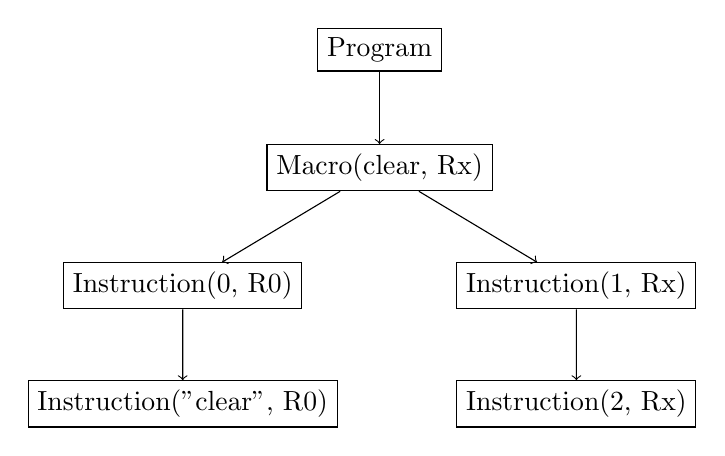
\begin{tikzpicture}[nodes={draw}, ->]

    \node{Program}[sibling distance = 5cm]
    child {node{Macro(clear, Rx)}
        child {node{Instruction(0, R0)}
            child {node{Instruction("clear", R0)}
                }}
    child { node {Instruction(1, Rx)} 
        child { node {Instruction(2, Rx)} 
            }}}
        ;
    \end{tikzpicture}
    \caption{Tree of the example code}
    \label{tree}
\end{figure}









\section{Interpreter}
\label{sec:interpreter}
The phase of interpretation is made after the parsing. 
An interpreter is made of an (hypothetical) infinite memory, a set of macros definitions and a list of instruction and three special registers:
\begin{itemize}
    \item $R_C$ $\rightsquigarrow$ the register counter that indicates the current instruction
    \item $R_0$ $\rightsquigarrow$ the input register
    \item $R_1$ $\rightsquigarrow$ the output register
\end{itemize}

\subsection{Internal representation of the memory}
The memory of the interpreter is represented by the \textit{RAM} class witch a class which extends the \textit{dict} class of Python.
This class redefines :
\begin{itemize}
    \item the \textit{getitem} method : if we try to access a not existing key of the \textit{dict}, it is firstly created with the $0$ value and then $0$ is returned. 
    \item the setitem method : which casts the value associated to the key as an \textit{Int}
\end{itemize}

\subsection{How the interpreter treats macros}
When the interpreter receives a list of instructions to be interpreted, it tries at first to remove every instruction that is a macro call. 
For example if we have a code like the following :
\begin{lstlisting}[
    caption={RAM code with macro representing the $\times 2$ operation}, 
    label={code_macro_times_two},
    mathescape, 
    frame=lines,
    backgroundcolor=\color{gray!10},
    ]
    begin macro times_two(Rx, Ry)
    Ry = Ry + 1
    Ry = Ry + 1
    Rx = Rx - 1
    end macro;
    R0 = R0 + 1
    times_two(R0, R1)
    if R0 $\neq$ 0 then gotob 1
    R1 = R1 - 1
    R1 = R1 - 1
\end{lstlisting}
\newpage
The interpreter will receive :
\begin{itemize}
    \item The macro name \textit{times\_two} which put $R0 \times 2$ in $R1$
    \item The list of 5 instruction :
    \begin{itemize}
        \item R0 = R0 + 1
        \item add\_reg(R0, R1)
        \item if R0 $\neq$ 0 then gotob 1
        \item R1 = R1 - 1
        \item R1 = R1 - 1
    \end{itemize}
\end{itemize}

At first, the interpreter reads every instruction and when it detects the 
\[\textit{times\_two(R0, R1)}\] 
macro call, it replaces that line by the body of the macro definition, where parameters of body of the the macro has been replaced by the macro call arguments.

It is important to note, that if we only perform this substitution, our code will be broken, since the jump inside \textit{IF} statements will not work as expected. 

In fact, when we make a macro-call replacement, we should always keep attention on the number of step to do and actually modify them.

The code of Listing \ref{code_macro_times_two} will be so replaced by the following one :

\begin{lstlisting}[
    caption={RAM code without macro representing the $\times 2$ operation}, 
    label={code_macro_times_two_no_macro},
    mathescape, 
    frame=lines,
    backgroundcolor=\color{gray!10},
    ]
    R0 = R0 + 1
    R1 = R1 + 1
    R1 = R1 + 1
    R0 = R0 - 1
    if R0 $\neq$ 0 then gotob 3
    R1 = R1 - 1
    R1 = R1 - 1
\end{lstlisting}

\subsection{A bug we still have in jump}

The code is able to correct the jump in \textit{IF} statements in the case where the \textit{IF}
\begin{itemize}
    \item is not inside a macro
    \item is inside a macro but it does not \textit{go out} from the macro body
\end{itemize}
\newpage
Let's look Listing \ref{listing:macro_bug}.

\begin{lstlisting}[
    caption={RAM code causing a bug}, 
    label={listing:macro_bug},
    mathescape, 
    frame=lines,
    backgroundcolor=\color{gray!10},
    ]
    begin macro macro_little_jump(Rx)
    if Rx != 0 then gotob 1
    end macro;
    macro_with_1000_lines(R10)
    macro_little_jump(R0)
\end{lstlisting}

In this example, we should notice that the jump inside the macro \textit{macro\_little\_jump} should be replaced by an \textit{IF} with a jump of $1000 + 1$ lines (the number of lines of \textit{macro\_with\_1000\_lines} + the original jump = $1$), but in reality the jump is not modified.

The macro with an \textit{IF} statement, in fact, only consider its own body definition.

Notwithstanding this, a code like in Listing \ref{listing:macro_working}, will work, since the \textit{IF} jump remains inside the macro scope and it will be corrected to a jump of $1001$ steps.

\begin{lstlisting}[
    caption={RAM code causing a bug}, 
    label={listing:macro_working},
    mathescape, 
    frame=lines,
    backgroundcolor=\color{gray!10},
    ]
    begin macro macro_little_jump(Rx)
    macro_with_1000_lines(R10)
    if Rx != 0 then gotob 1
    end macro;
    macro_little_jump(R0)
\end{lstlisting}

\subsection{Interpretation of instructions}
Once we have ended the macro substitution process, we can finally compute our instructions one by one or the whole program till

\[ R_C = 0\; \lor\; R_C> |instructions| \]

via the \textit{execute} method on every \textit{Instruction}.

We are allowed to get the state of the memory of our program at every moment via the \textit{memory} attribute of the \textit{Interpreter} or get the output (that is $R_1$) thanks the \textit{get\_output} method.
\newpage
\subsection{Predefined macros}

The interpreter knows some predefined macros :
\begin{itemize}
    \item \textit{push $R_k$} which pushes the the content of $R_k$ in a very big register ($2^{64}$)
    \item \textit{pop $R_k$} which takes the value from register $2^{64}$ and puts it in $R_k$
    \item \textit{rp($R_x$, $R_y$)} which takes the \textit{right part} of $R_x$ and put it in $R_y$
    \item \textit{lp($R_x$, $R_y$)} which take the \textit{left part} of $R_x$ and put it in $R_y$
\end{itemize}

\subsection{Parsed object to Interpreter one}

In Sections \ref{sec:parser} we have said that parser needs chained lists to create step by step the object that will be returned after the parsing. On the other hand, for reason of time complexity, the interpreter must work with normal list since accessing the \textit{i-th} element should be as fast as possible. We know that getting the last element of a chained list takes a linear time, whereas in a \textit{Python} list the time needed should be almost constant.

Therefore, after the parsing phase, it is necessary to operate this transformation so that the interpreter can work.

The \textit{parser\_instr\_to\_interp\_list} function in \textit{pars\_to\_interp.py} file does exactly this task.

We create a \textit{list} $L$ of instruction and a \textit{dictionary} $D$ of macros and then we go through the chained list. So, if we find a \textit{macro} definition we add it to the $D$ and if we find an \textit{instruction} then we will append it into $L$.





\section{Graphic interface}

\begin{figure}%
    \centering
    \subfloat[\centering Menu file]
    {{\includegraphics{images/menu/menu_file.png} }}%
    \qquad
    \subfloat[\centering Menu help]
    {{\includegraphics{images/menu/menu_help.png} }}%
    \qquad
    \subfloat[\centering Menu run]
    {{\includegraphics{images/menu/menu_run.png} }}%
    \qquad
    \subfloat[\centering Menu tools]
    {{\includegraphics{images/menu/menu_tools.png} }}%
    \qquad
    \subfloat[\centering Menu option]
    {{\includegraphics[width=5cm]{images/menu/menu_option.png} }}%
    \caption{Menu previews}%
    \label{fig:menu_images}%
\end{figure}

\subsection{Menu bar}
On the menu bar we can find :
\begin{itemize}
    \item \textbf{File}:
    \begin{itemize}
        \item \textit{New File} : Open a new blank file into a new tab (with an ephemeral default name, until you save it).
        \item \textit{Open File} : Choose and open an existing file with your OS file browser and load it.
        \item \textit{Save} : Save the current file on the disk. If it is a new created file, the name and save location will be asked.
        \item \textit{Exit} : Quit the application. Be careful to previously save
        your unsaved files before performing this action.
    \end{itemize}
    \item \textbf{Run}:
    \begin{itemize}
        \item \textit{Start} : Begin the sequential execution of the current file. This means that you start executing the first instruction, then you manually execute each of the following instructions. The program stops as soon as the last instruction has been executed.\\
        \textit{Remark: this command will be disabled if the sequential execution has already been started.}
        \item \textit{Run Next Instruction} : Execute the next instruction of the program.\\
        \textit{Remark: this command is disabled if the sequential execution hasn't already been started.}
        \item \textit{Run All Instructions} : Execute all the next instructions of the program. The delay between two execution is 0.1 sec.\\
        \textit{Remark: this command is disabled if the sequential execution hasn't already been started.}
        \item \textit{Run File} : Execute the whole file in one go.
    \end{itemize}
    \item \textbf{Stop}: Interrupt the current sequential execution. Memory will be reset.\\
    \textit{Remark: this command is disabled if the sequential execution hasn't already been started.}
    \item \textbf{Tools}:
    \begin{itemize}
        \item \textit{Apply Preprocessing} : Modify the current file by executing only the preprocessing instructions (\#define and \#include). It is useful
        when we got an error to see the involved line or to see the final program which will be parsed.
        \item \textit{Cantor Encode} : Open a utility window in which you can convert two integers to one with the Cantor's function.
        \item \textit{Cantor Decode} : Like the previous command, but the reverse function.
    \end{itemize}
    \item \textbf{Options}: Open the settings window in which we can check/uncheck:
    \begin{itemize}
        \item Show the lines numbers of the text editor
        \item Automatically open the executed code's window
        \item Automatically open the memory's window
        \item Put the default value 0 if there is no R0 entry
    \end{itemize}
    You have to confirm to save and apply your choices. These will be saved on an JSON file.
    \item \textbf{Help}:
    \begin{itemize}
        \item \textit{Get Started}: Open an window in which the main command are explain. This is a user manual.
        \item \textit{RAM instructions}: Explanation of the four different RAM instructions.
        \item \textit{About}: Developers of the application.
    \end{itemize}
\end{itemize}

\subsection{Icons bar}

\begin{figure}[h]%
    \centering
    \includegraphics{images/menu/menu_icons.png}%
    \caption{Icon bar}%
    \label{fig:icon_bar}%
\end{figure}

The icon bar (Figure \ref{fig:icon_bar}) is composed of four icons. The first one is a shortcut to save the current file. The second run the whole file, the third start the sequential execution and the last is the Stop shortcut.

\subsection{Text editor}

This widget is where you can write and edit your code. This is also here the file you open will be loaded.
Line numbers are displayed to the left of the text entry field.

\subsection{Entry}

You can set the value of the R0 register when you run the program. If no value is entered, an error message will be displayed, except if you set the adequate option.
\subsection{Displayers}
Two windows are available to see and debug your RAM program. The first (\textit{Display Executed Code}) displays all the instructions after the preprocessing and parsing phases. If you execute a code sequentially, the last executed instruction will be highlighted. Since then, you can easily see and debug the progress of the program.

The second one (\textit{Display Memory}) will display the state of the memory (registers). Equally, the memory will be actualize to each iterations.
Each window is assigned to a file.
\subsection{Output console}
It is in this terminal that you will see the file execution's result. Error messages will also be displayed there.
If the program contains a grammatical error or an unrecognized instruction, the file will not be interpreted and the number of the line on which the said error appears will be displayed. Attention, this is the line corresponding to the preprocessed file.
You can adjust the space taken by it easily by hovering the mouse just below the widget where the code is inserted, as you would with a window.
\subsection{Shortcuts}
Several shortcut allow you to perform action quickly.

\underline{Inside the text editor:}
\begin{itemize}
    \item \textbf{\textit{Ctrl+Shit+Enter}} : Run whole file.
    \item \textbf{\textit{Ctrl+Enter}} : Start sequential execution.
    \item \textbf{\textit{Ctrl+M}} : Run all instructions sequentially.
    \item \textbf{\textit{Right-Click}} : Show contextual menu.
\end{itemize}
Depending on whether you are in RAM program or Int code mode, the right-click contextual menu changes.\\
In \textbf{RAM Program mode}, you can mark a line as the end of file when you run it. You can remove the marker.
You also have the possibility of executing the file directly from this contextual menu.\\
In \textbf{Int Code mode}, you will be offered to convert the file that contains the int to a RAM program in a new tab, or you can directly execute the int.


\underline{On the main window:}
\begin{itemize}
    \item \textbf{\textit{Ctrl+S}} : Save the current file.
    \item \textbf{\textit{Ctrl+O}} : Open file.
    \item \textbf{\textit{Ctrl+N}} : Create new file.
    \item \textbf{\textit{Esc}} : Exit
\end{itemize}


\begin{figure}[t]%
    \centering
    \subfloat[\centering Main panel]
    {{\includegraphics[width=8cm]{images/gui.png} }}%
    \qquad
    \subfloat[\centering Memory panel]
    {{\includegraphics[width=4cm]{images/memory.png} }}%
    \caption{Example of our graphic interface}%
    \label{fig:gui}%
\end{figure}


\section{Distribution of tasks}
The distribution of the tasks was done relatively naturally according to our respective affinity. Antoine made the graphic part, Davide the interpreter, Margaux the parser and Federica the help panel. 

\section{Summary}
Finally, we have a version of our application in which most of the requirements of the specifications have been implemented. You can interpret a RAM program or directly an integer. If the program is not correct, the user will be warned. It is quite easy to use the software.

Although this application is complete, we could consider some graphical improvements like open a folder and display it in the tree explorer on the left, as in the traditional text editor. More ambitious would be create an editor that able to do automatic completions and suggest syntactic corrections. From a back-end point of view, we could improve our interpreter by taking into account a jump which exceeds the context of a macro.

This project allowed us to finally understand what is the basis of any computer and any program. it was very formative and gave us a lot of perspective.
\appendix

\begin{appendices}
\addtocontents{toc}{\protect\setcounter{tocdepth}{0}}

\section{Grammar}
\label{grammar}

program ::= code
 
code ::= \\
\tab expression code \\
\tab | expression \


expression ::= \\
\tab "R" number "=" "R" number "+" number \\
\tab | "R" number "=" "R" number "-" number \\
\tab | "if" "R" number "!=" number "then" "gotob" number \\
\tab | "if" "R" number "!=" number "then" "gotof" number \\
\tab | "push" "R" number \\
\tab | "pop" "R" number \\
\tab | "rp" "(" listRegister ")" \\
\tab | "lp" "(" listRegister ")" \\
\tab | name "(" listRegister ")" \\
\tab | "begin" "macro" name "(" macroListRegister ")" macroCode "end" "macro"";" 

listRegister ::= \\
\tab "R" NUMBER "," listRegister \\
\tab | "R" NUMBER \\
\tab | 

macroListRegister ::= \\
\tab "R" name "," macroListRegister \\
\tab | "R" name \\
\tab | 

macroCode ::= \\
\tab macroExpression macroCode \\
\tab | macroExpression 

macroExpression ::= \\
\tab macroId "=" macroId "+" number \\
\tab | macroId "=" macroId "-" number \\
\tab | "if" macroId "!=" number "then" "gotob" number \\
\tab | "if" macroId "!=" number "then" "gotof" number \\
\tab | "push" macroId \\
\tab | "pop" macroId \\
\tab | "rp" "(" listMacroId ")" \\
\tab | "lp" "(" listMacroId ")" \\
\tab | name "(" listMacroId ")" \\
\tab | "begin" "macro" name "(" macroListRegister ")" macroCode "end" "macro"";" 

macroid ::= \\
\tab "R" name \\
\tab | "R" NUMBER 

listMacroId ::= \\
\tab macroId "," listMacroId \\
\tab | macroId \\
\tab | 

name ::= \\
\tab STRING ( NUMBER | STING )*


\end{appendices}

\end{document}